\section{Methods}
\label{sec:methods}
% How do I approach it?
In terms of analysis subjects with huge varieties, data registration is an important step.
Registration could be approached in different perspectives.
First, registration on image, which uses image intensity as a major feature, has being developed in medical image analysis for past decade. 
Hill et al. and Sotiras et al. wrote very educated review articles on this topic~\cite{hill2001medical,otiras2013deformable}.
On the other hand, registration on shape, which uses geometric cues as major feature, has succeeded in many applications in computer vision and computer graphics fields~\cite{belongie2002shape,li2012temporally}.
However, applying such techniques for aligning pediatric airway data was still a hard problem.
Hong et al. proposed a simplified airway model which is much easier to register for further analysis~\cite{hong2014statistical}.

% Need to familiar with
\subsection{Simplified airway model}
\label{sec:simplified_airway_model}
In this work, I applied Hong et al.'s simplified airway algorithm.
The algorithm first segments the airway from CT images using Otsu-thresholding and two manually chosen seeds that bracket the upper airway.
Then the upper airway can be approximated by a centerline with cross sections.
The centerline is inferred based on the heat distribution along the airway flow that is solved by a Laplace equation.
Cross sections are cut from segmented airway geometry using planes that are orthogonal to the centerline. 
The area of the cross sections would be the 1D functional data representation of an airway.

\subsection{Landmark detection}
\label{sec:landmark_detection}
Once we have functional data, we can register them alone with some common landmarks across subjects.
Typically the landmark annotation was performed manually.
For reducing the manually annotation cost, based on Dalal and Triggs's  detection framework~\cite{dalal2005histograms}, I propose a landmark detection framework using concatenating Histogram of Gaussian (HOG) features and geometric prior.

The first step in the framework is to train a binary classifier using concatenating HOG.
HOG is well designed normalized local histograms of image gradient orientation in a dense sample grid.
The original purpose of this feature was for human detection.
Nevertheless, it captures edge or gradient structure that is very characteristic of local shape, and it can be efficiently computed.
For applying HOG on 3D image, instead computing histogram is arbitrary 3D orientation, I attempted to computed 2D HOG in axial, coronal, and sagittal plane, which are the three perspectives for user annotations.
This reduced the computational complexity and made learning feasible given limit amount of ground truth annotations.
In prediction stage, the trained classifier can be applied to the particular landmark it was designed for.
Figure~\ref{fig:detection} illustrated detection of trachea carina (TC).

\begin{figure}[tb]
  \begin{center}
    \begin{tabular}{ccc}
    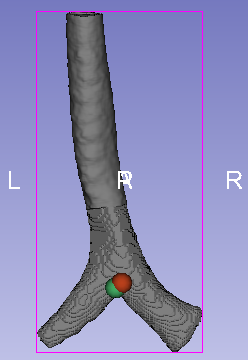
\includegraphics[height=34.5mm] {fig/Fleck_005_geometry.png}
    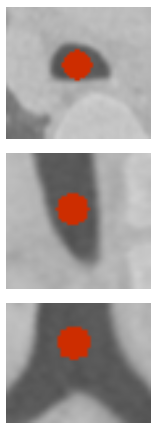
\includegraphics[height=35mm] {fig/landmark.png}
    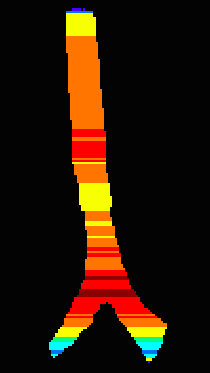
\includegraphics[height=34.5mm] {fig/Fleck_005_likelihood.png}
    \end{tabular}
    \caption{ \label{fig:detection} Visualization of the framework of landmark detection. First, an airway geometry is segmented by Otsu-thresholding. Green marker is the ground truth annotation and red marker is the predicted location of TC. Second, concatenating HOG features are computed in the center of trachea in each depth. From top to down: Sagittal, coronal, and axial. Final, applying the trained classifier on these different hypotheses to get likelihoods of the landmark. Dark red indicates the highest likelihood of TC. In this case, the predicted TC has only 1.97 mm (the total length is 159 mm) away from the ground truth annotation. This error is only 1.2$\%$ of the entire airway.
    }
  \end{center}
\end{figure}

After landmarks are located, we can register the functional data to the unified domain~\cite{ramsay2006functional}.
In Hong et al.'s original paper, each subject had five visible landmarks from nasal spine, choana, epiglottis tip, true vocal cord (TVC), and TC.
In our dynamic data, most of subjects only have TVC and TC.
Even thought, in some cases, TC is the only available landmark which makes alignment impossible using current approach.
Then, a heuristic assumption would be applied to these special cases.
The assumption is the subject has the same length of trachea from TVC to TC with the most relevant subject (in terms of age) in our data.
Therefore, we can compute the portion of the existed trachea by measuring the ratio of the length of current trachea in physical space and the length of the most relevant subject from TVC to TC.

\subsection{Statical atlas analysis}
\label{sec:statical_atlas_analysis}
Given special aligned functional data I would like to capture population changes with respect to some factors, say age.
A kernel regression approach can achieve the objective by assigning weights to data-object with respect to age.
For example, I used Gaussian weight function $w_i(a_i; \sigma, \bar{a}) = c\exp{(a_i-\bar{a})/2\sigma^2}$, where $a_i$ is the age for the observation $i$, $\sigma$ is a predefined standard deviation and $c$ is the normalization constant for fitting data to a specific age.

To further analyze the weighted data, I applied weighted functional boxplots to build statical atlas for each dynamic subject~\cite{hong2013weighted}.
Functional boxplots was originally proposed by Sun and Genton~\cite{sun2011functional} which requires a definition of band depth for functional data.
Here I used a weighted version to fit the population changes.

Band depth is a rank of functional data for ordering it from the center outward. 
Basically, the idea is the more subsets to which a data is belonged, the more centrality that data might have.
Given a set of functional data $Y=\{y_i | i=1,...,n\}$, a combinatorial function $C$ which enumerates all two pair combinations in a set, and a band function $B(y_1, y_2) = \{(t,x(t)): t\in \mathrm{T}, \mathrm{min}(y_1(t),y_2(t)) \leq x(t) \leq \mathrm{max}(y_1(t),y_2(t))\}$,
the band depth $D$ of a functional data $y$ with respect to a set $Y$ can be defined as

\begin{equation}
D(y; Y) = \sum_{y_i, y_j \in C(Y)} I[y \subset B(y_i, y_j)],
\label{eq:band_depth}
\end{equation}
where $I$ is an indicator function.
A general version of band depth is weighted modified band depth

\begin{equation}
D'(y; Y) = \sum_{y_i, y_j \in C(Y)} w_iw_j\lambda[ B(y_i, y_j) ]
\label{eq:weighted_band_depth}
\end{equation}
where $\lambda$ is the Lebesgue measure, and $w$s are the weights of kernel regression.
The measurement of membership of a functional data is relax in 
(\ref{eq:weighted_band_depth}), and it is based on a weighted populations which fits our objective.

When a rank of functional data is available, we can compute interesting statics such as median, interquartile range, and outliers of the population.
I applied (\ref{eq:weighted_band_depth}) to compute population atlas and plot subject dynamics upon the population atlas using (\ref{eq:band_depth}).